\section{Implementation and evaluation}\label{sec:schemeTest}
This section describes the implementation issues and results obtained by implementing the dynamic packet length control scheme defined in section \ref{sec:DPLC} and testing it in a real scenario. The implementation is done on TelosB motes. For the test of the scheme, two different programs are written: One for a transmitter mote and for a receiver mote. 
\paragraph{Transmitter} The transmitter is the more complicated of the two motes. First, it is initiated with $l_0 = 10$, $l_1 = 20$ and $\mathcal{E}_0 = 0$. It will then send out messages of the given payload length periodically, every $50$ milliseconds, i.e. $20$ messages per second. The transmission power of the mote is set to $-15$ dBm, according to level $7$ in TinyOS. After $100$ messages have been transmitted, it will request the receiver how many packets it received. The request is repeated infinitely, untill an answer is received from the receiver mote. Upon receiving an answer, the transmitter mote estimates the current transmission efficiency, and calculates a new packet length according to the result and figure \ref{fig:d}, where the threshold $D$ is set to $0.1$, which corresponds to a $1 \%$ change in channel efficiency. If the change was less than this, the packet length remains the same, and the transmitter is considered in steady state. After the channel has been in steady state for $15$ seconds, a change of $l_i = l_{i-1} +10$ is forced, unless the payload size is already at maximum, where $l_i = l_{i-1} - 10$ instead. The payload length is constrained to be $l_i \in \{10, 20, ... , 100\},\forall i$.
\paragraph{Receiver} The receiver mote is also programmed to fit the specificed functionality. It is initiated with a counter of $0$, which is incremented each time a packet from the transmitter mote is received. Upon receiving the request for the counter, the receiver formats a message containing only the count. As the transmitter mote will keep resending the request untill it receives the answer, the receiving mote keeps the count and answers with it untill it receives a message that is no longer a request. When this happens, the counter is reset. Further, the receiver mote is connected to a laptop through a serial connection, reporting the payload length of the messages it received, as to be able to monitior the dynamic change in payload length.
\\[8pt]
In a first experiment to see how the scheme performs, the two motes are set up $35$ meters apart in an indoor environment. They are placed such that line of sight propagation is possible. According to the previous estimation of the same channel, described in section \ref{sec:chanEst}, shown on figure \ref{fig:35mTest}, the optimum payload length is approximately $80$-$100$ bytes. Therefore, the scheme is expected to converge to roughly these values. 
The result of recording the behavior of the payload size for the first six minutes is shown on figure \ref{fig:35mDPLC}. It is seen that the scheme is initiated with a small payload size, and immediately increases to a payload length of $80$ bytes. The size then fluctuates between $60$ and $90$ bytes for the first half of the five minute period. Then, eventually, the size changes and the payload size is $90$ or $100$ bytes for the remaining time. This could easily be caused by a change in the characteristics of the channel. A histogram for the full measurement, $8$ minutes of the payload lengths are shown on figure \ref{fig:35mHist}. This is useful to visualize the frequency of each payload length, showing what the most used lengths are. In this experiment, $l=100$ bytes is by a good margin the most used length, followed by $l=90$ bytes. This is in accordance with the expectations from the experiment in section \ref{sec:chanEst}.
\\[8pt]
A second experiment is made, this time with a larger distance between the motes, $45$ meters. It is expected for the channel to perform worse, as was also observed in the initial experiment in section \ref{sec:chanEst}. It was observed from figure \ref{fig:45mTest} that the optimum payload length should likely be in the range of $50$-$90$ bytes. The result of the first six minutes of the experiment is shown on figure \ref{fig:45mDPLC}. It is seen that once again the scheme starts out at a small packet size, but immediately increases it. The increase stops at $60$ bytes, where a steady state is found. After maintaining the steady state for $3$ time steps, the scheme again searches for a better payload length, finding a new steady state at $70$ bytes. An interesting observation is that around five minutes the channel conditions seem to improve for a little while, and the scheme does indeed adjust to this, but reduces back down when the conditions becomes worse again. A histogram of the entire seven minute experiment is shown on figure \ref{fig:45mHist}. It is seen that the most frequently used payload lengths are $60$, $70$ and $80$ bytes. These three lengths account for $76\%$ of transmitted packets, fitting the expectations well. 
\begin{figure}
\centering
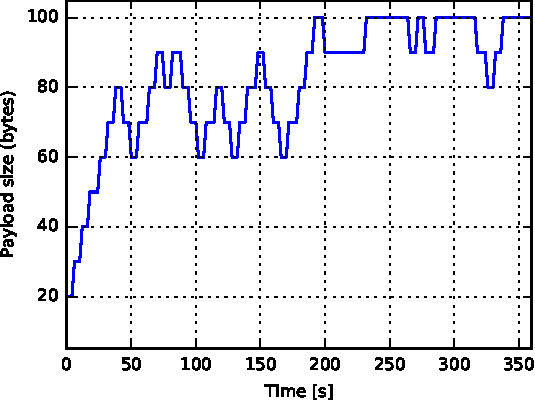
\includegraphics[scale=1]{figs/35mDPLC.pdf} 
\caption{\textit{Dynamic changes of payload length over time, 35 meters apart}\label{fig:35mDPLC}}
\end{figure}
\begin{figure}
\centering
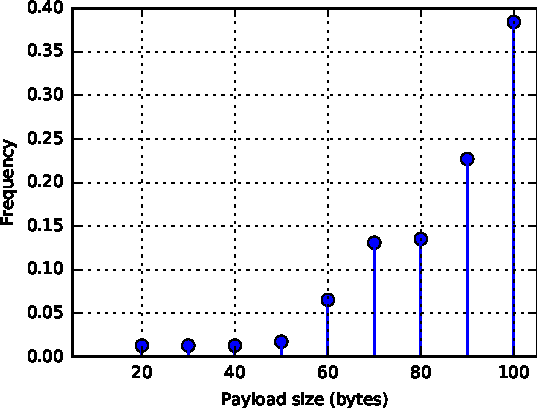
\includegraphics[scale=1]{figs/35mHist.pdf} 
\caption{\textit{Frequency of payload lengths used, 35 meters apart}\label{fig:35mHist}}
\end{figure}
\begin{figure}
\centering
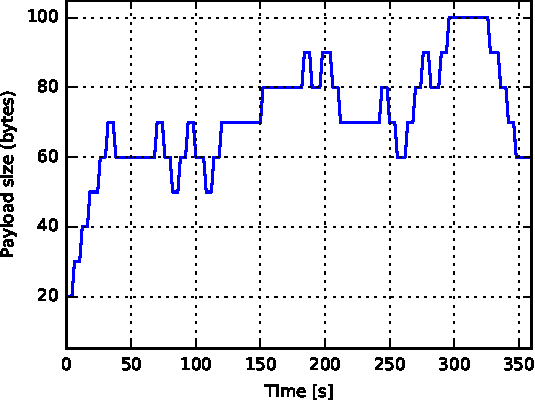
\includegraphics[scale=1]{figs/45mDPLC.pdf} 
\caption{\textit{Dynamic changes of payload length over time, 45 meters apart}\label{fig:45mDPLC}}
\end{figure}
\begin{figure}
\centering
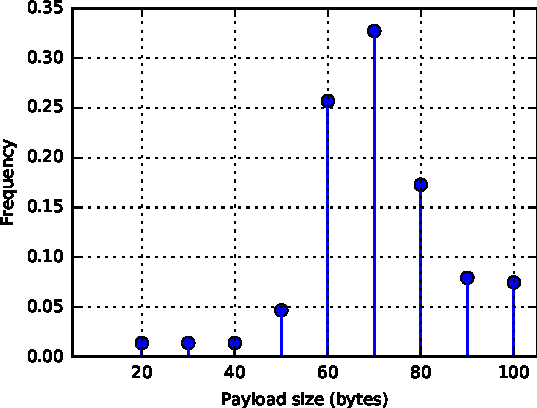
\includegraphics[scale=1]{figs/45mHist.pdf} 
\caption{\textit{Frequency of payload lengths used, 35 meters apart}\label{fig:45mHist}}
\end{figure}